\chapter{DSOA}
\label{ch:3}
Neste capítulo apresentaremos a plataforma DSOA (\textit{Dynamic SOA}), dando uma visão geral da motivação e dos objetivos da plataforma. Apresentaremos também uma rápida descrição dos principais componentes que constituem a arquitetura da plataforma, contextualizando a realização deste trabalho.

\section{Contexto e Objetivos}
\label{sec:dsoa_intro}

A natureza dinâmica e distribuída do ambiente SOA e o não-determinismo dos atributos de qualidade sugerem a necessidade de um sistema de monitoração contínua.

Nesse contexto, a plataforma DSOA estende as capacidades fornecidas pelas arquiteturas orientadas a componentes baseados em serviços atuais, com a capacidade de adaptação dos componentes em função dos atributos de qualidade. 

Esse tipo de arquitetura é na verdade um modelo de composição de serviços, onde temos as figuras do consumidor e do provedor de serviços, nitidamente separadas.

Neste cenário, a adaptação faz sentido em ambos os lados. No lado do consumidor de serviços, a adaptação consiste na capacidade de selecionar serviços de funcionalidade equivalente, com ciência da qualidade provida. No lado do provedor, essa adaptação faz sentido a medida que existe a necessidade de garantir aspectos de qualidade anunciados.

Assim, o objetivo de DSOA é propor uma plataforma orientada a componentes baseados em serviços que estende a capacidade do \textit{container}, de forma a tratar com aspectos de QoS, em particular, aspectos relacionados a desempenho.

Neste sentido, tratar aspectos de qualidade relacioanados a desempenho é um objetivo desafiador, pois, a maioria das plataformas existentes, não dão suporte a isso. O mais próximo disso, podem ser vistos no iPOJO~\cite{ipojo}, \textit{Declarative Services}~\cite{declarative} e BluePrints~\cite{blueprint}. Porém, tais plataformas tratam apenas de aspectos relacionados a questão da disponibilidade do serviços, não considerando aspectos de desempenho.

\section{Arquitetura}
\label{sec:dsoa_arch}

Como vimos na Seção \ref{sec:dsoa_intro}, no contexto da adaptação dinâmica, a consideração de atributos de qualidade ligados a desempenho traz a necessidade de monitoramento constante de tais atributos. Para isso, torna-se necessária a figura de um sistema de monitoração \textit{online}. Basicamente, um sistema de monitoração é composto por uma linguagem de especificação (para definir configurações de monitoração), um conjunto de sensores (para coletar dados), analisadores e processadores de eventos (para realização de ações com base na análise dos dados monitorados). 

Uma representação desse tipo sistema pode ser vista na Figura \ref{fig:monitor}.


\begin{figure}[htp]
\centering
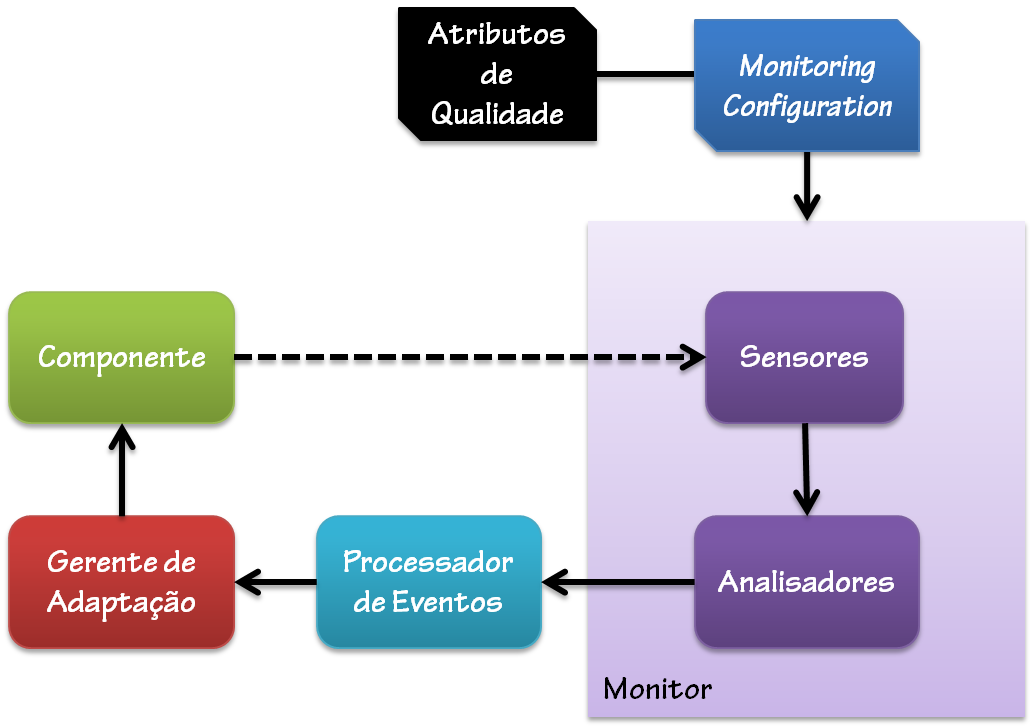
\includegraphics[width=11cm]{chapters/chapter3/monitor.png}
\caption{Sistema de Monitoração}
\label{fig:monitor}
\end{figure}

Porém, para prover adaptação dinâmica, o \textit{container} deve ser capaz de modificar-se sem provocar a interrupção do serviço. Deste modo, a plataforma especifica a inclusão de uma camada de serviços de utilidade sob a camada de composição de serviços e uma camada de adaptação sobre a mesma, visando estender suas capacidades, conforme a Figura \ref{fig:dsoa_arch}.

\begin{figure}[htp]
\centering
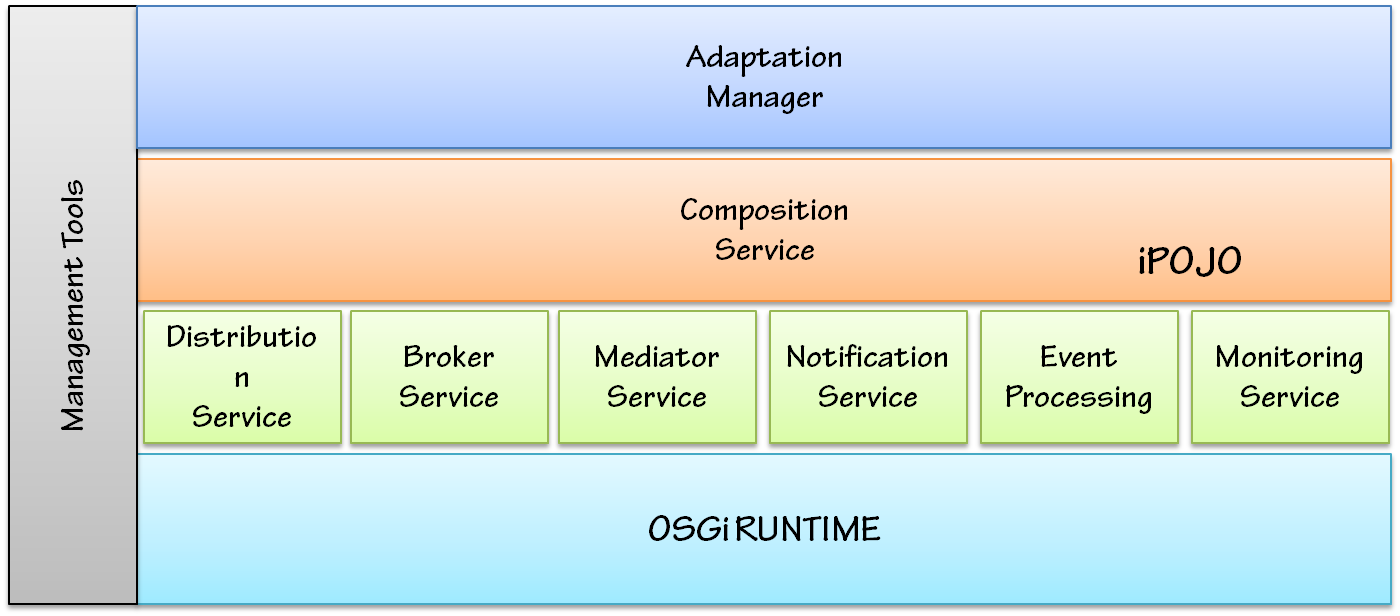
\includegraphics[width=13cm]{chapters/chapter3/dsoa-arch.png}
\caption[Arquitetura em Camadas DSOA]{Arquitetura em Camadas DSOA.}
\label{fig:dsoa_arch}
\end{figure}

\subsection{Componentes}
Nesta seção, daremos uma visão geral de cada componente presente na arquitetura, identificando sua funcionalidade e suas características principais.

\subsubsection{\textit{Distribution Service}}
\label{subsub:dosgi}
O serviço de distribuição é responsável por permitir que serviços disponibilizados no registro do \textit{runtime} OSGi local sejam distribuídos como serviços remotos a outros \textit{runtimes}. Esse serviço é provido através da utilização do DOSGi~\cite{dosgi}, que implementa um conjunto de serviços que provêem distribuição de serviços OSGi. Seu funcionamento baseia-se na idéia de um registro centralizado de serviços remotos, descritos como \textit{endpoints}, onde esses serviços são disponibilizados localmente através de ~\textit{proxies} que permitem o acesso ao ~\textit{endpoint}.

\subsubsection{\textit{Adaptation Manager}}

É o principal componente da arquitetura e é responsável por gerenciar dinamicamente as dependências das aplicações, com base em atributos de qualidade. 

No ambiente DSOA, uma aplicação pode ser vista como uma composição de serviços sendo especificada de forma declarativa, ou seja, cada composição possui um descritor, no qual são indicadas as interfaces dos serviços necessários e os atributos de qualidade esperados. Nesse contexto, cabe ao gerente de adaptação interpretar este descritor e buscar garantir que os serviços selecionados para a composição atendam aos critérios de qualidade especificados. Caso isso não ocorra, cabe a ele, adaptar dinamicamente a aplicação substituindo o serviço em uso, por um mais adequado.

Outra responsabilidade do \textit{Adaptation Manager} é solicitar ao serviço de monitoração a verificação da qualidade do serviço provida pelos elementos da composição, através da definição de configurações de monitoração (\textit{monitoring configurations}).

\subsubsection{\textit{Broker Service}}
O \textit{broker service}  provê um mecanismo de seleção de serviços com base em atributos de qualidade. Ele abstrai a busca ao registro para o gerente de adaptação e através de um conjunto de serviços de seleção especializados em atributos de qualidade, retorna os serviços que melhor atendem as necessidades do consumidor.

As necessidades do cliente são definidas em tempo de ~\textit{deployment} através de propriedades do componente. Porém, todo o processo de seleção e adaptação é realizado dinamicamente em tempo de execução. 


\subsubsection{\textit{Mediator Service}}
Fornece um serviço de integração e mediação de serviços distribuídos, com funcionalidades equivalentes em diversas tecnologias, a partir de uma interface única, que media a invocação a estes serviços. O esquema de mediação é definido através de uma interface gráfica que realiza o cadastro das interfaces do serviço concreto e das interfaces de integração de serviços.

\subsubsection{\textit{Notification Service}}
O serviço de notificação é responsável por sinalizar as quebras de contrato ao gerente de adaptação, permitindo que este tome as medidas necessárias para garantir os aspectos de qualidade esperados. As notificações são realizadas através do envio de eventos assíncronos, baseado no padrão de troca de mensagens \textit{publish-subscribe}, definindo tópicos para a publicação e entrega de notificações por meio de eventos.

\subsubsection{\textit{Event Processing Service}}
\label{subsec:cep}
O serviço de processameto de eventos é o módulo responsável pelo processamento dos eventos que ocorrem na plataforma. Em particular, a própria infra-estrutura gera eventos relacionados ao ciclo de vida dos serviços, representando, por exemplo, o envio de requisições e respostas, a publicação e a remoção de serviços, além de eventos derivados que indicam o nível de qualidade do serviço percebido pela aplicação. Ele também é responsável pela verificação de quebras de contrato, através da análise dos dados de qualidade recebidos. 

Em termos de complexidade computacional, esta é uma tarefa extremamente custosa, sobretudo pela quantidade de eventos que devem ser processados. Deste modo, o serviço é implementado sob uma \textit{engine} de processamento de eventos complexos, \textit{Esper}~\cite{esper}, que fornece um mecanismo de processamento de \textit{stream} de eventos e uma linguagem de consulta própria (\verb EQL ), facilitando o processamento configurável dos eventos em tempo real, através da criação de \textit{statements} que selecionam ou correlacionam dados provenientes do processamento dos eventos.

\subsubsection{\textit{Monitoring Service}}
\label{subsec:monit_serv}
O serviço de monitoração é responsável por inicializar a monitoração dos serviços utilizados pela aplicação. Ele recebe as configurações de monitoração, extraídas através das especificações do serviço pelo \textit{adaptation manager}, e configura o \textit{Event Processing Service} de maneira a processar os eventos gerados pela monitoração dos atributos de qualidade da aplicação.

É função do serviço de monitoração, definir os \textit{statements} utilizados no processamento de eventos. Estes \textit{statements} são construídos com base nas \textit{monitoring configurations} repassadas pelo \textit{adaptation manager}.

\subsubsection{\textit{Composition Service}}
DSOA utiliza o iPOJO~\cite{ipojo} como infra-estrutura à composição de serviços. Ele implementa um \textit{container} que realiza a injeção de dependências na aplicação, ou seja, indica quais serviços devem ser utilizados na composição, sob uma pespectiva puramente funcional. Assim, temos na figura do \textit{adaptation manager} e dos demais serviços, uma extensão da infra-estrutura de suporte à composição, permitindo o uso de atributos de qualidade na seleção dos serviços que deverão compor a aplicação.

\subsubsection{\textit{Management Tool}}
Este componente fornece um conjunto de ferramentas administrativas para gerenciar a plataforma e os serviços que estão em execução, intergradas a VisualVM~\cite{visualvm}, uma ferramenta visual para gerenciamento de aplicações na plataforma Java SE.

\section{Considerações Finais}
Este capítulo apresentou a plataforma DSOA, que um conjunto de componentes na forma de serviços, para lidar com atributos de qualidade visando a adaptação dinâmica da aplicação. Assim, os conceitos apresentados neste capítulo são essenciais para a contextualização deste trabalho, uma vez que, este tem como um dos objetivos, estender a plataforma conforme veremos no próximo capítulo.